\chapter{Szczegóły Implementacyjne}
\label{chapter-4}

\section{Użyte narzędzia}

\noindent Projekt inżynierski został napisany zaimplementowany jako program komputerowy w języku python. Do realizacji zostały użyte głównie paczki:

\begin{itemize}
    \item numpy- paczka służąca do obliczeń naukowych. Udostępnia rozbudowane API do algebry liniowej i przetwarzania sygnałów.
    \item scipy- moduł umożliwiający obliczenia matematyczne i techniczne, w szczególności przetwarzanie sygnałów stosowane w tej pracy
    \item matplotlib- paczka służąca do wizualizacji danych.
    \item rir generator- moduł umożliwiający symulację odpowiedzi impulsowej pokoju
\end{itemize}

\noindent Więcej informacji można znaleźć w dokumentacji paczek \cite{numpy}, \cite{matplotlib}, \cite{rir} i \cite{scipy}.

\section{Metologia rozwoju programu}

\noindent Realizacja pracy była podzielona na stworzenie właściwego programu opisane szczegółowo w rodziale \ref{chapter-3} i na stworzenie generatora symulującego rzeczywisty sygnał mikrofonowy z dodatkiem zakłóceń.


W założeniach oprogramowanie miał mieć charakter obiektowy. Główne bloki zostały zaimplementowane jako klasy, które komunikują się między sobą za pomocą interfejsów. Takie rozwiązanie powoduje usystematyzowaną strukturę projektu i umożliwia łatwy rozwój oprogramowania w przyszłości. Przykładem jest implementacja algorytmu MUSIC. Klasa MUSIC dziedziczy po klasie abstrakcyjnej DOA. W ten sposób proste w przyszłości będzie dopisanie w programie innego algorytmu estymacji kierunku nadchodzenia fali jako innej klasy dziedziczącej po DOA. Poniżej przedstawiono diagram klas w konwencji UML \cite{uml}:

\begin{figure}[h!]
    \centering
    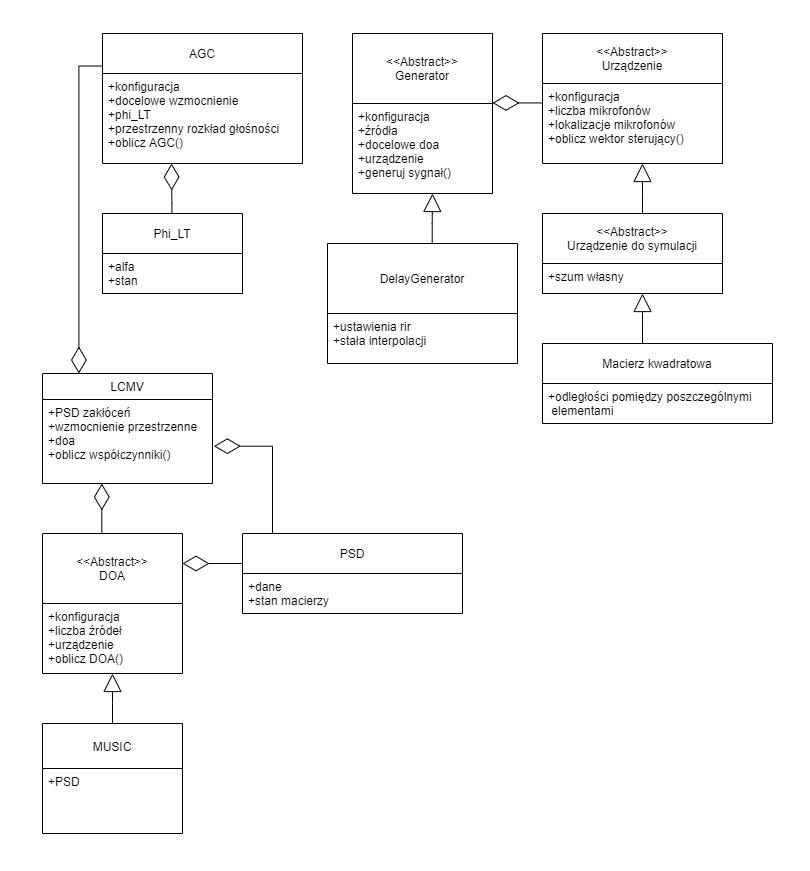
\includegraphics[width=\textwidth]{Images/uml_pl.png}
    \caption{Diagram Klas}
    \label{fig:classes}
\end{figure}


\noindent W diagramie \ref{fig:classes} skrótowo opisano klasy. Nazwy nie odpowiadają( poza DelayGenerator) nazwom w kodzie. Nie są również dodane wszystkie składowe i metody. Schemat ma za zadanie przedstawić koncepcyjnie zaimplementowane rozwiązanie i pokazać podejście autora pracy do implementacji systemu.


\newpage

\section{Generator}

Generator pełni ważną rolę w projekcie inżynierskim. Z tego powodu postanawia się poświęcić mu osobną sekcję w tekście. 

\noindent Generator przyjmuje jako wejścia następujący dane:

\begin{itemize}
    \item Obiekt macierzy mikrofonowej
    \item Sygnały dzwiękowe 
    \item Funkcję kąta w czasie
    \item Funkcję wzmocnienia w czasie
    \item Opcjonalnie informacje o geometrii pokoju i o tym czy symulacja pogłosu jest włączona
\end{itemize}

\noindent Schemat działania generatora jest względnie prosty. Przyjmuje się model przedstawiony w rozdziale \ref{chapter-2}. Zakłada się, że sygnał wejściowy odpowiada wartości sygnału w punkcie $\bm{\mathrm{d}}_{0}$. Posiłkując się równaniami \eqref{equation:2.4} i \eqref{equation:2.5} można zapisać, że:

\begin{equation}
    \label{equation:delay model}
    \mathrm{x}_{l}(\bm{\mathrm{d}}_{m},t) = 
    \mathrm{x}_{l}(\bm{\mathrm{d}}_{0},t-\tau)
\end{equation}

\noindent Gdzie $\mathrm{x}_{l}(\bm{\mathrm{d}}_{m},t)$ to wymuszenie $l$-tej fali dzwiękowej w punkcie $\bm{\mathrm{d}}_{m}$. W takim układzie możliwe są bieżące zmiany opóźnienia bazując na pozycji źródła. Dodatkowo możliwa jest generacja białego szumu $n(t)$. Biały szum o mocy $\sigma$ może być przedstawiony jako zmienna losowa z rozkładu gaussowskiego o średniej 0 i wariancji $\sigma$.

\noindent Generator umożliwia symulację pomieszczenia, w  którym znajduje się mikrofon. Za pomocą paczki rir generator \cite{rir} generowana jest odpowiedź impulsowa pokoju $\bm{\mathrm{h}}(t)$. Tak generowana odpowiedź nazywana będzie później pogłosem. Szczegóły dotyczące genezy takiego sposoby symulacji pomieszczenia mogą być znalezione w książce \cite{Kuttruff}. Ostatecznie zatem sygnał wejściowy na $m$-tym mikrofonie może być zapisany w dziedzinie czasu jako:

\begin{equation}
    \label{equation:full generator}
    \mathrm{x}(t,\bm{\mathrm{d}}_{m})=
    \sum_{l=1}^{L}
    \mathrm{x}_{l}(\bm{\mathrm{d}}_{0},t-\tau_{l,m})*
    h_{l}(t)+ n(t)
\end{equation}

\noindent Z uwagi na to, że w celu generacji filtra pogłosowego konieczne są konkretne pozycje źródeł i mikrofonu, włączenie symulacji pomieszczenia nie pozwala na zmiany pozycji źródeł w czasie symulacji.




\section{Schemat przetwarzania danych}

Algorytm przetwarza nagrane pliki dzwiękowe. Składa się z następujących kroków:

\begin{algorithm}
  
  \caption{Schemat przetwarzania}
  \begin{algorithmic}[1]
    \State Na wejście trafia M ścieżek dzwiękowych
    
    \State Sygnał jest przetwarzany do reprezentacji STFT
    
    \State Przetwarzanie odbywa się w pętli po kolejnych indeksach czasowych, nazywanych ramkami
    
    \State Na wyjściu przetwarzania sygnałów zwracany jest sygnał $Y(k,n)$ jako STFT
    
    \State Dane wyjściowe są przetwarzane za pomocą odwrotnej krótkoczasowej transformaty fouriera (ISTFT) do postaci czasowej.
    
  \end{algorithmic}
\end{algorithm}

\begin{figure}[h!]
    \centering
    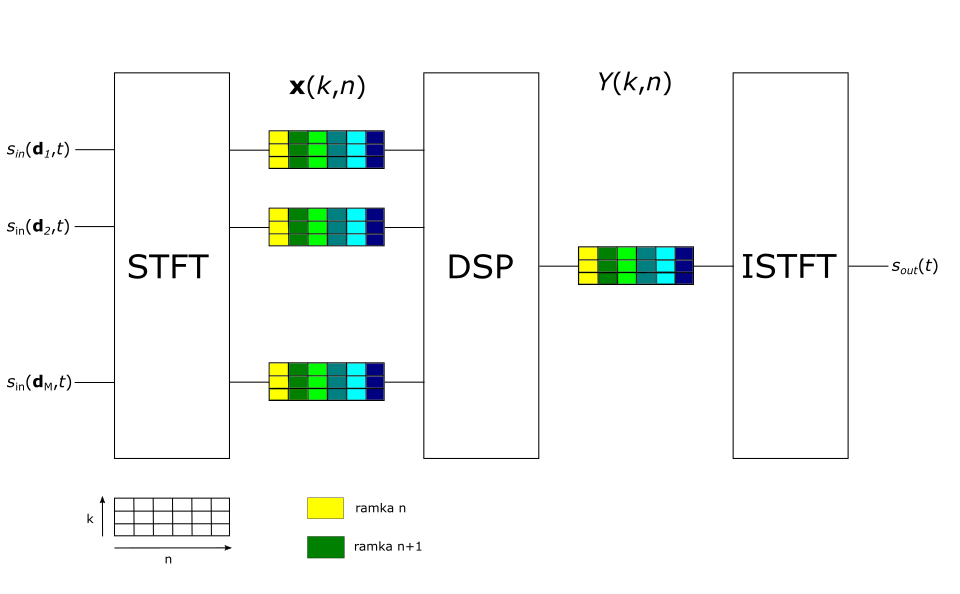
\includegraphics[width=\textwidth]{Images/processing.png}
    \caption{Schemat przetwarzania}
    \label{fig:processing}
\end{figure}

\noindent Na rysunku \ref{fig:processing} blok oznaczony jako automatyczna kontrola głośności zawiera w sobie operacje obliczenia PSD, estymacji DOA, wyznaczania współczynników i filtracji przy użyciu LCMV. Jest więc równoznaczny z diagramem \ref{fig:block_diagram}.

